\chapter{Data}

\section{Probability Distibution to Find Particles $P(x)$}

\begin{figure}
  \centering
  \begin{subfigure}{.45\textwidth}
    \centering
    \includegraphics[width=\textwidth]{./data/plots/distrib-mit.pdf}
    \caption{With Laser, $\sigma_\text{t} = \num{0.1351}^{+0.0049}_{-0.0046}\si{\um}$}
  \end{subfigure}
  \begin{subfigure}{.45\textwidth}
    \centering
    \includegraphics[width=\textwidth]{./data/plots/distrib-ohne.pdf}
    \caption{Without Laser, $\sigma_\text{f} = \num{0.0771}^{+0.0028}_{-0.0026}\si{\um}$}
  \end{subfigure}
  \caption[Tracked Location of single Particles]{\textbf{Tracked Location of single Particles}, both a free and a trapped particle are recorded using the digital microscope. The particles' locations are tracked over all frames using \textit{Blender} and marked as a dot each. In total, the positions in 402 frames at 13 fps are shown for each particle.}
	\label{fig:distrib}
\end{figure}

\begin{figure}
  \centering
  \includegraphics[width=\textwidth]{./data/plots/mostly-linear-fit.pdf}
  \caption{This should be linear, $m = \SI{1.403e-03}{\um\squared\per\second}$}
\end{figure}

Multiple free particles and one trapped by the laser are located on the microscope slide and a \num{30} second video clip is recorded.
The free sofware \texttt{Blender} is used to track the motion of the particles and save the positions for later evaluation as the provided software sucks. \todo{rephrase}
The aquired positions of the free patricles are used to find the diffusion coefficient $D$ as established in \autoref{sec:brown}.

For visualization, the positions $\vec{x}(t)$ of a free particle and the trapped patricle are marked in scatter plots shown in \autoref{fig:distrib}.
The trapped particle should move less than the free particle.
However this cannot be observed on the recorded data, possibly because the slide was already slightly dried out, so many of the observed particles did not move as freely anymore.

The pdf is given by a 2D gaussian:
\begin{equation*}
	P(\vec{x}) = \frac{1}{Z} \text{e}^{-\frac{U(\vec{x})}{\text{k}_\text{b} T}}
\end{equation*}

Modelling the potential as a harmonic potential $U(\vec{x}) = \frac{1}{2} D \vec{x}^2$ gives a function
\begin{equation}
	P(\vec{x}) = \frac{1}{Z} \text{e}^{-\frac{\vec{x}^2}{2 \sigma}},
\end{equation}
which is fitted to the two datasets using a likelihood method.
The parameters found are $\sigma_\text{f} = \num{0.0771}^{+0.0028}_{-0.0026}\si{\um}$ for the free particle and $\sigma_\text{t} = \num{0.1351}^{+0.0049}_{-0.0046}\si{\um}$ for the trapped particle.

Contrary to the expected decrease in motion for the trapped particle, the trapped particle's probability density is more spread than that of the free particle.
This could be explained by localized heating by the laser, though it is likely not the reason as both the fluid and the \textbf{BALLS}$^{^\text{hah}}$ \todo{Remove humor} are transparent.
More likely the observed free particle was held stationary by some form of friction.

\section{Maximum Trapping Force}
The maximum trapping velocity $v_\text{max}$ is determined by moving the particle at an increasing velocity while it is trapped until it slips away.
A value of
\begin{equation*}
	v_\text{max} = \SI{30(10)}{\micro\meter\per\second}
\end{equation*}
is observed.
The vast error on the velocity is justified by the assumption that the slide could have been dried out, effectively increasing the friction force and, hence, lowering the maximum velocity.
Utilizing \autoref{eq:max_trap}, it follows that
\begin{equation*}
	F_\text{max} = \frac{4k_\text{B}T}{m}\cdot v_\text{max} = \SI{805.2(1178)}{\pico\newton},	%http://www.wolframalpha.com/input/?i=%5Cfrac%7B4*Boltzmann+constant+*+297+K%7D%7B6.111e-04+um%C2%B2%2Fs%7D*30+um%2Fs
\end{equation*}
so the observed value lies within the expected order of magnitude.

The errors on $m$, $v_\text{max}$ and $T$ propagate into the error on $F_\text{max}$ like
\begin{equation*}
	\Delta F_\text{max} = \sqrt{\left(\frac{4k_\text{B}v_\text{max}}{m}\right)^2\cdot\left(\Delta T\right)^2 + \left(\frac{4k_\text{B}T}{m}\right)^2\cdot\left(\Delta v_\text{max}\right)^2 + \left(\frac{4k_\text{B}Tv_\text{max}}{m^2}\right)^2\cdot\left(\Delta m\right)^2},
\end{equation*}
where we assumed an error of $\Delta T = \SI{2}{\kelvin}$ on the temperature.

The maximum velocity is dependent on the viscosity of the used medium.
Higher viscosities mean lower values of $v_\text{max}$ and vice versa since the trapping force remains constant at a constant intensity.
If the particles had been suspended in ethanol ($\eta_\text{dyn} = \num{1.2}\text{cP}$)\footnote{\label{ref:viscosity}\url{https://hydramotion.com/uploads/view/20160224144736_Hydramotion_Viscosity_Units.pdf}} instead of water ($\eta_\text{dyn} = \num{1}\text{cP}$)\footnoteref{ref:viscosity}, a lower value for $v_\text{max}$ would have been measured.
\section{ink stuff}
A slide is prepared with a line of red and black felt-tip marker, alcohol is added as a solvent.
The slide is placed under the microscope and the laser is turned on on it's highest power setting.
Different effects are observed for both colors.

The black marker stripe looks uniform before turning on the laser.
The areas hit by the laser become lighter that their surroundings, the laser can be used to draw shapes.

The red marker stripe is not uniform, the pigment is distributed in a cell-like structure.
Turning on the laser causes the individual cells to merge.

\begin{figure}
  \centering
  \begin{subfigure}{.45\textwidth}
    \centering
    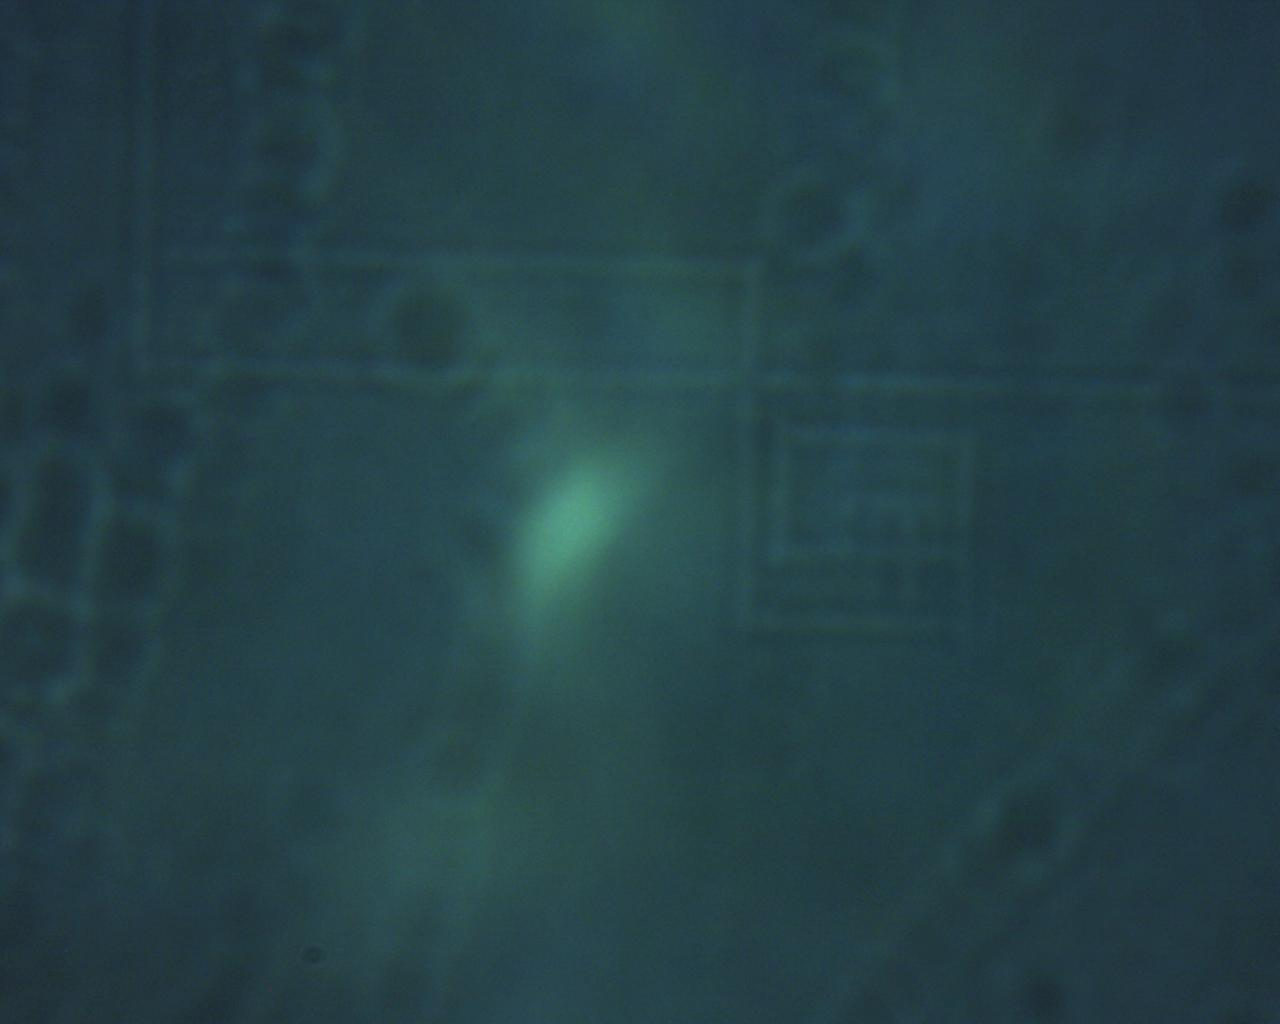
\includegraphics[width=\textwidth]{./data/source/schwarz.jpg}
    \caption{black permanent marker with spiral pattern drawn by laser}
  \end{subfigure}
  \begin{subfigure}{.45\textwidth}
    \centering
    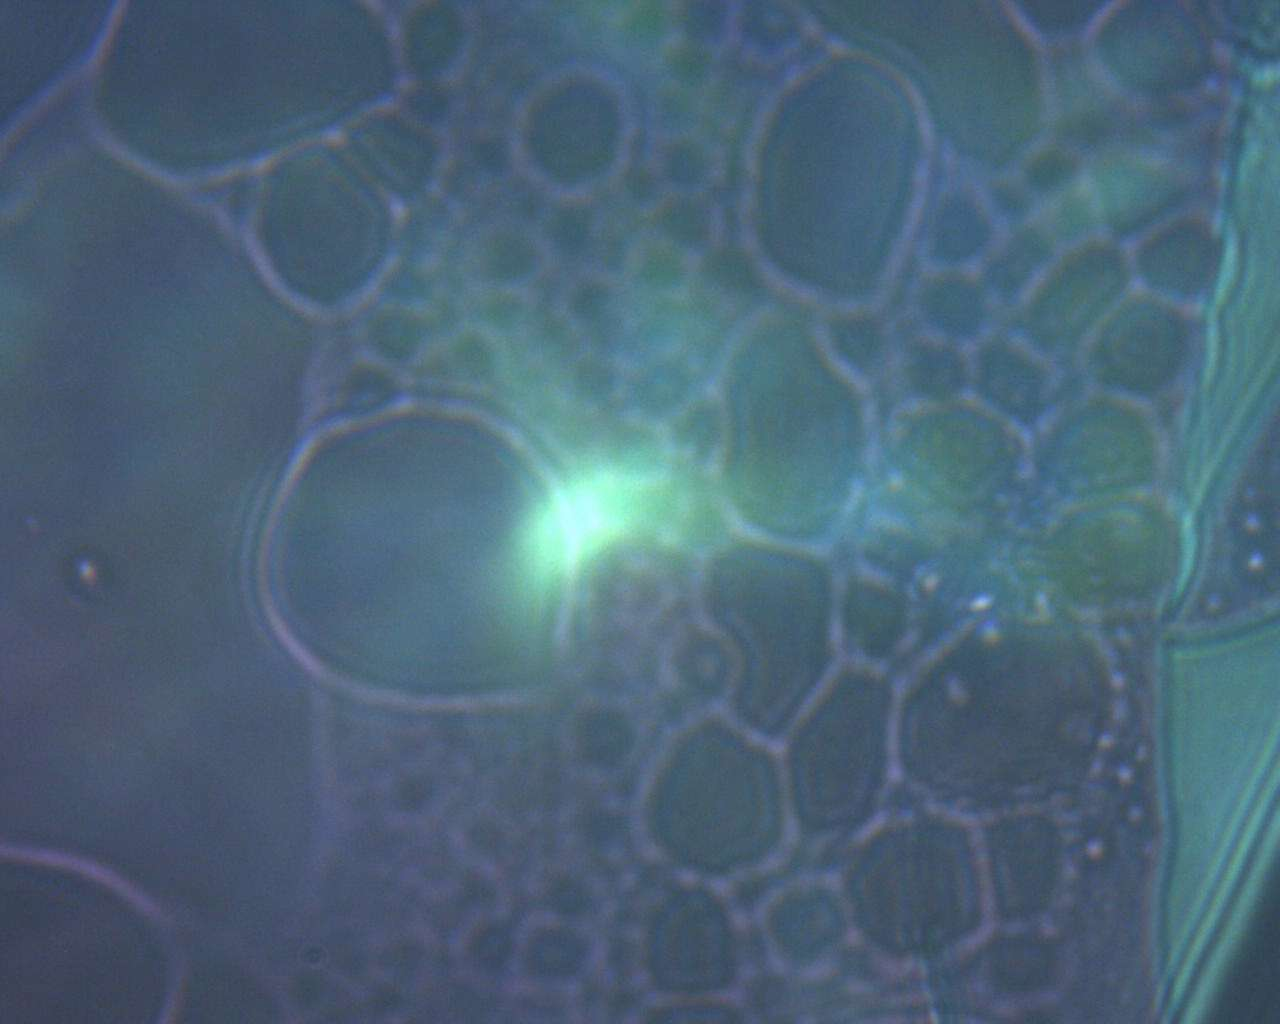
\includegraphics[width=\textwidth]{./img/red-before.jpg}
    \caption{red dry-erase marker before turning on the laser}
  \end{subfigure}
  \begin{subfigure}{.45\textwidth}
    \centering
    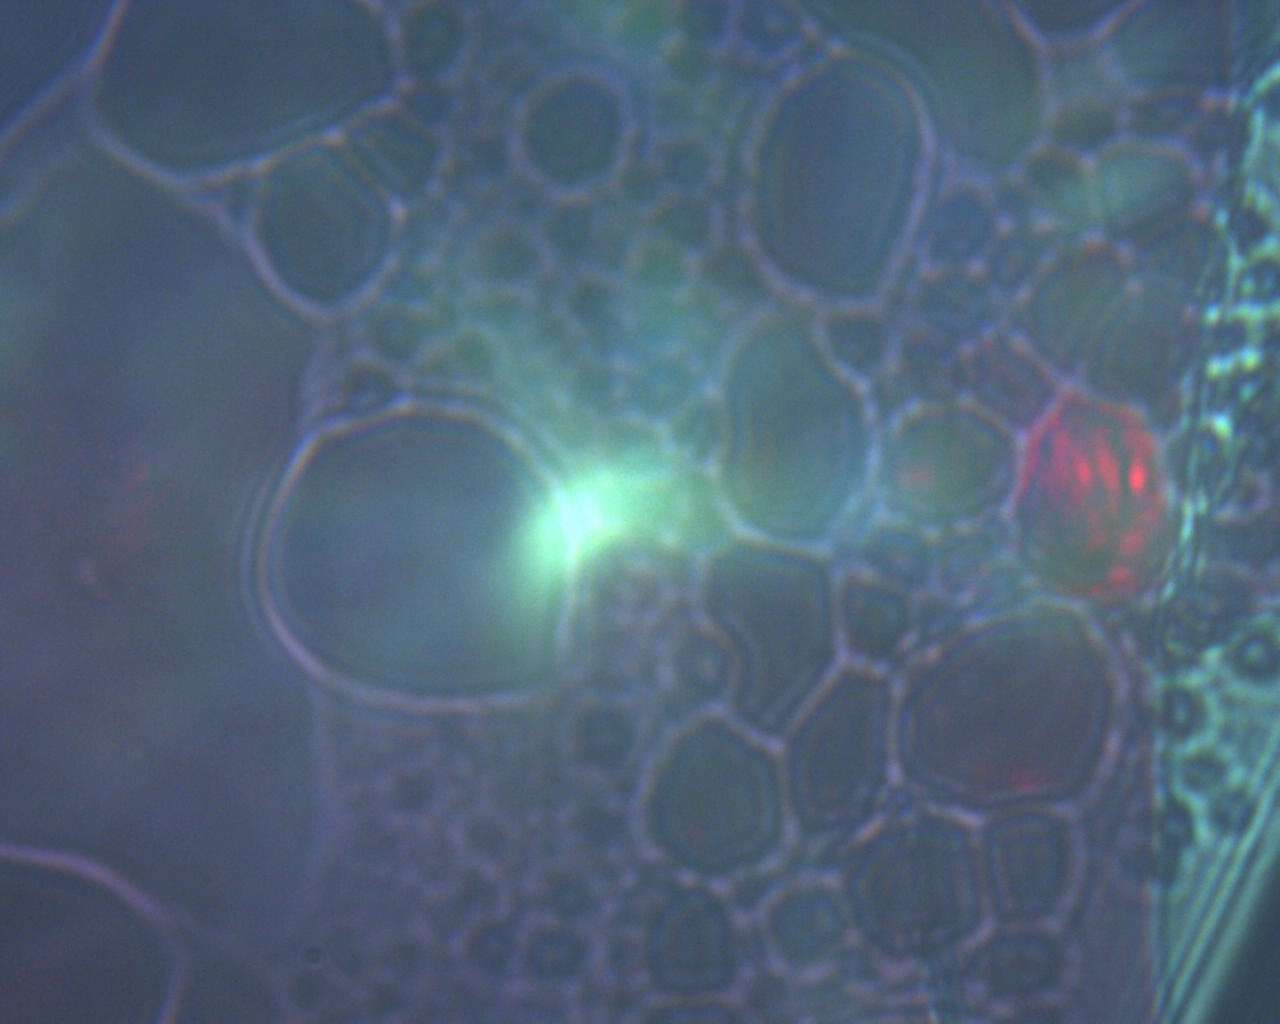
\includegraphics[width=\textwidth]{./img/red-1.jpg}
    \caption{red dry-erase marker immediately after turning on the laser}
  \end{subfigure}
  \begin{subfigure}{.45\textwidth}
    \centering
    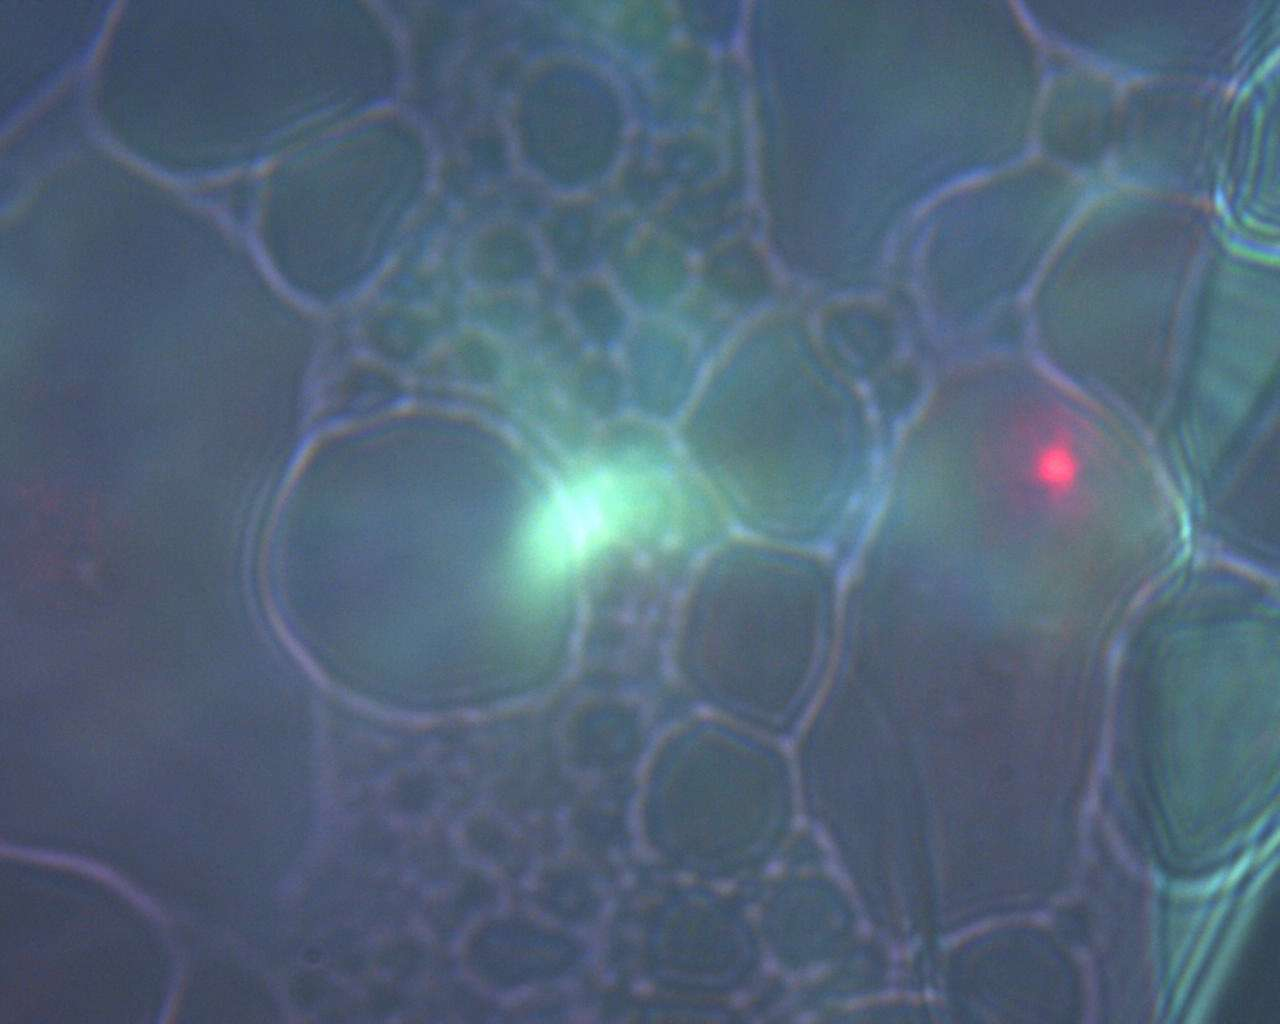
\includegraphics[width=\textwidth]{./img/red-2.jpg}
    \caption{red dry-erase marker \SI{\approx 20}{\s} after turning on the laser}
  \end{subfigure}

  \caption[Ink under laser]{\textbf{Ink under laser}, \num{114} microns across full width}
\end{figure}
